\documentclass[a4paper,10pt]{article}
\usepackage[utf8]{inputenc}
\usepackage[margin=0.5in]{geometry}
\usepackage{amsmath}
\usepackage{xfrac}
\usepackage{listings}
\usepackage{graphicx}
\usepackage{wrapfig}
\usepackage{adjustbox}
\graphicspath{{figures/}}


%opening
\title{JAnalysisTools Manual}
\author{J. T. Smallcombe}
\begin{document}

\maketitle
\tableofcontents

\section{Introduction}
This library designed to help working with root for analysis contains several GUI analysis tools and useful sets of functions. An explanation of some of the major components is given here, but subclasses and functions will not be detailed.
Within the GUI classes hover over any control to view explanatory tooltip text.
Various histogram presentation formating and automated fitting macros (for spectroscopic peaks and detector efficiency curves) are also included and may be documented later. 

\section{Install}
This library has only been tested with ROOT6, it does not currently have any other non-standard dependencies.
Source the ROOT6 $thisroot.sh$.
In the base directory of the library run:
\lstset{language=bash}
\begin{lstlisting}
make clean
make -j 4
source bin/thisjlib.sh
root -l bin/root_start.C
\end{lstlisting}
If all worked well root started without error messages and is running with the library loaded.
For future use add a source of $thisjlib.sh$ to your bashrc and add $gSystem->Load("libJanalysistools.so")$ to your root startup script.

\section{jEnv Toolbar}
A graphical session manager toolbar to handle grabbing (selecting) of histograms with no typing.
To create a new instance simply type:
\lstset{language=C++}
\begin{lstlisting}
new jEnv();
\end{lstlisting}
in a ROOT interactive session. A new window will open:
\renewcommand{\labelenumi}{\Alph{enumi}}
\begin{center}
\begin{tabular}{ c c }
\begin{minipage}{0.7\textwidth}
\begin{enumerate}
\item Grabbed Histogram Icon
\item Open a new peak fitting environment (copy grabbed histogram if $TH1$)
\item Open a new 2/3D gating tool if grabbed histogram is $TH2/TH3$.
\item Open a new TBrowser and draw grabbed.
\item Create a new canvas and draw a copy of grabbed
\item Open a dialogue box to save grabbed to disk
\item Close the toolbar.
\item Exit root
\item Open/Close the AddSub Tool panel.
\end{enumerate} \end{minipage}
&
\raisebox{-.5\height}{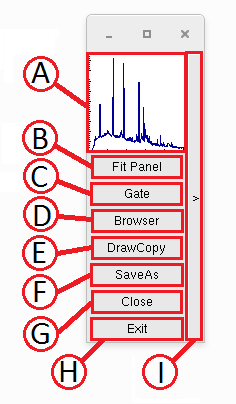
\includegraphics[width=0.23\textwidth]{jEnvA.png}}
\\
\end{tabular}
\end{center}

%\begin{wrapfigure}{r}{0.25\textwidth}
%\end{wrapfigure}
\subsection{Histogram Grabbing}
Whenever an instance of jEnv exists histogram grabbing is enabled in all $TCanvas$s, including those embedded in other classes/windows. Whenever a window containing a drawn histogram is clicked, a pointer to the first histogram of the frame is grabbed by jEnv and the small "Selected Histogram" icon will change. If a frame contains multiple histograms and you must click exactly on the desired histogram itself, not on the whitespace.

\begin{figure*}[!h]
\centering
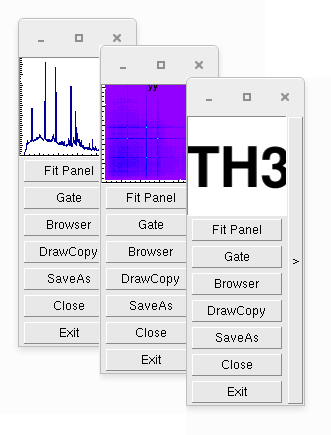
\includegraphics[width=0.3\textwidth]{jEnvB.png}
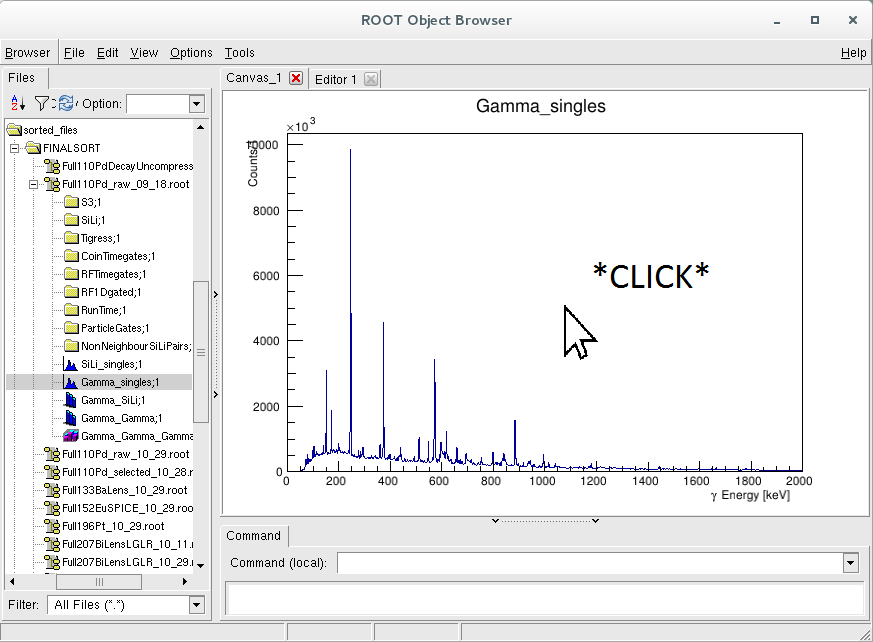
\includegraphics[width=0.52\textwidth]{jEnvD.png}     
\end{figure*}

Once a histogram is grabbed a copy of it will be passed to any of the functions of jEnv.

\subsubsection{Histogram Lifetime}
A histogram can go out of memory scope in several ways. For speed, as grabbing is done on EVERY canvas click, only a pointer is stored. jEnv will refuse to do anything with its histogram pointer until it has established it is valid. To check if a histogram is still in memory jEnv checks the histogram against roots list of object, however this object search has limitations. If this histogram is still drawn in the same canvas as when it was grabbed, it will be found.

\subsection{Histogram AddSub Tool}
Hidden in the side of jEnv is the AddSub tool. This is a simple tool to allow quick addition and subtraction of $TH1$s from anywhere. The tool even allows histograms with different binning, summing is done based on "user coordinates".
Click either of the selected histograms windows $A$ or $B$ to assign the currently grabbed histogram from jEnv, at this point a copy IS saved. The projected histogram is then given by $A\pm B*f$ where f is the fraction specified by the slider. In the case of subtraction the area of B is first normalised to that of A. The resultant histogram can also be grabbed.

\begin{center}
\begin{tabular}{ c c }
\begin{minipage}{0.4\textwidth}
\begin{enumerate}
\item Open/Close the AddSub Tool panel.
\item Subtraction/Addition fraction $f$ slider.
\item Selected Histogram A window/button
\item Swap A B
\item Selected Histogram B window/button
\item Fraction $f$ text entry.
\item Change between Subtraction/Addition.
\item Hide/Show error bars when drawing.
\item Result Window.
\end{enumerate} \end{minipage}
&
\raisebox{-.5\height}{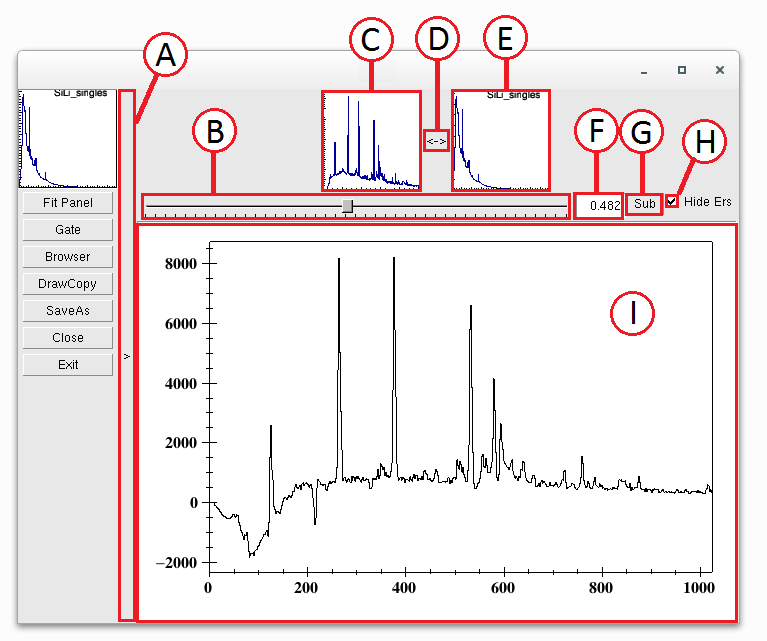
\includegraphics[width=0.55\textwidth]{jEnvC.png}}
\\
\end{tabular}
\end{center}

\section{Gating and Background Subtraction Tool}
The gating tool is designed to provide live graphical gating and background subtraction for $TH2$ and $TH3$ histograms filled with any data. 
A new instance can be created from the jEnv toolbar or typing any of the following:
\lstset{language=C++}
\begin{lstlisting}
new jgating_tool();
new jgating_tool(TH2*/TH3*);
new jgating_tool(HistogramName);
\end{lstlisting}
where "HistogramName" is the name (not title) of a histogram open in memory. The call with no arguments will grab the most recently selected or drawn histogram. If no valid input is found a window will not appear. Please wait a moment for the window to appear when using $TH3$s, particularly if they are large.
\begin{center}
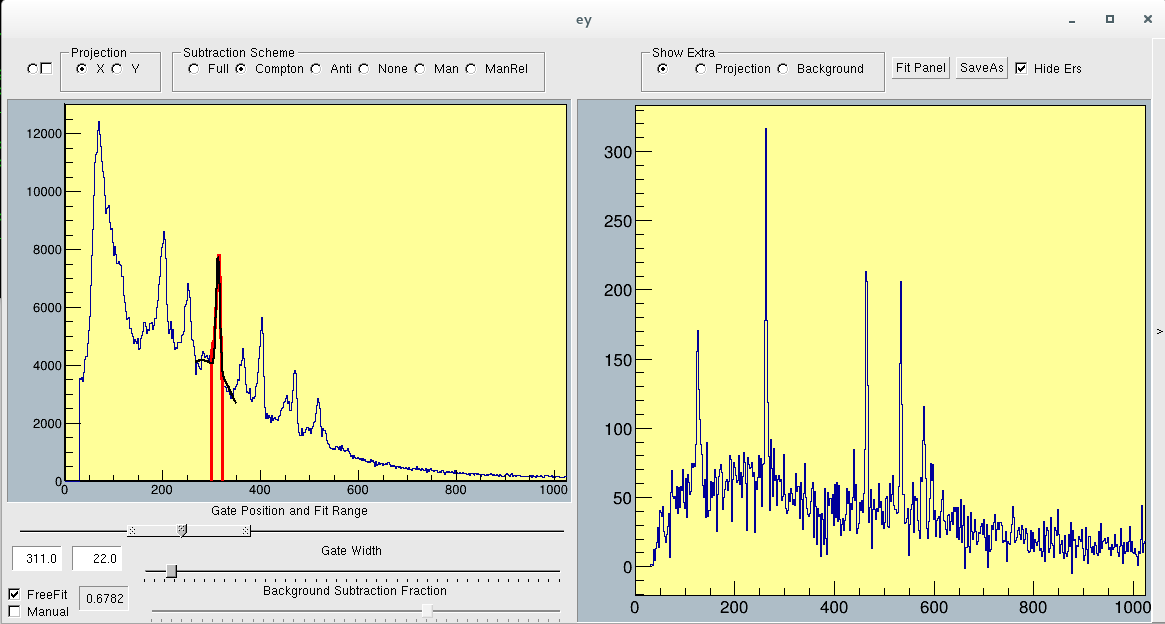
\includegraphics[width=0.55\textwidth]{jGateG.png}
\end{center}

\subsection{Gating Window}

\begin{center}
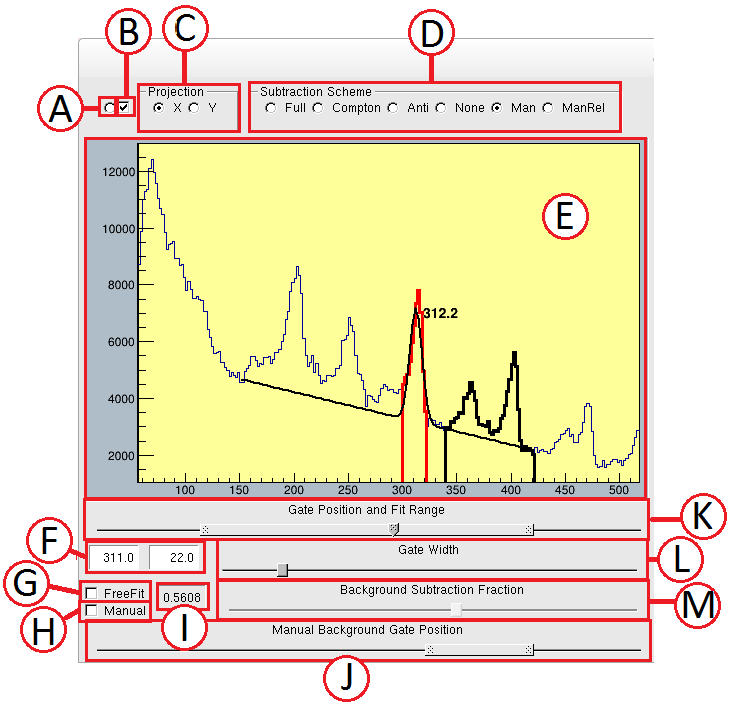
\includegraphics[width=0.5\textwidth]{jGateB.png}
\end{center}
\begin{enumerate}
\item Overflow Peek - By default shown projection excludes the overflow bins of the other axis. Hold this button to see the projecting including overflow overlain  
\item Show/Hide peak marker - By default text is shown indicating the centroid of the fitted peak.
\item Axis Select - Change the axis on which gating performed. (USE TO RESET IF ERRORS OCCUR)
\item Background Subtraction Type
\item Projection Window - Window showing the current projection and gate, when appropriate shows also fit and background gate. You can double click in this window to move the gate.
\item Gate Width and Centre - These act as both text entry boxes and outputs for the sliders. Both are in user coordinates but inputs will be rounded to bin multiples. 
\item Free Fit - The initial peak fit to determine background fraction is not a true fit as the background is a pol1 fixed by the user's cursor. Free fit fits a pol2 and will automatically fit a shrunk range in the presence of other peaks, useful for scanning.\raisebox{-0.9\height}{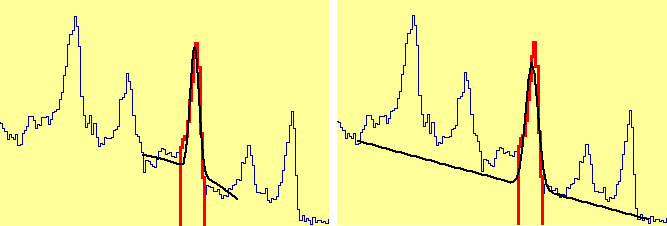
\includegraphics[width=0.4\textwidth]{jGateD.png}}
\item Enable Manual Background Fraction - Select this to enable manual adjustment of the background subtraction fraction, this will hide the peak fit.
\item Background Fraction Text Box - This can be used as a text entry box when manual background fraction is enabled.
\item Manual Background Gate - If manual background gate is selected, adjust the ends of this slider to define background gate (shown in black). This slider is hidden when not in use.
\item Gate \& Fit Slider - Use the central slider to adjust the position of your gate. When the fit is enabled, use the outer edges of the slider to adjust the range of the fit relative to the gate position.
\item Gate Width Slider
\item Background Fraction slider - Can be used to manually adjust background fraction, when manual background fraction is enabled.
\end{enumerate}

\subsubsection{Background Subtraction Type}
\begin{enumerate}
\item Full - This mode takes the full projection of the target axis as the background spectrum. A good first approximation in situations where a background cannot be clearly defined.
\item Compton - Background spectrum is formed by gating on the entire spectrum, including overflow, above the gate. Forms the best statistically sampled background spectrum for $\gamma$-ray gating. The background starts 2 bins above the gate or 2$\sigma$ if the fit is used. If directly adjacent to a spectrum dominating peak this may not be the best option. 
\item Anti - The background gate is the entire spectrum excluding the data gate.
\item None - No subtraction.
\item Man - User specified manual gate. When selected an additional slider will be displayed and the selected gate will appear in the gating window. If the background gate encompasses the data gate that region will be excluded.
\item ManRel - Relative position manual gate. As Man but the background gate will move when the data gate moves. Useful for scanning.
\end{enumerate}

\subsection{Result Window}
\begin{center}
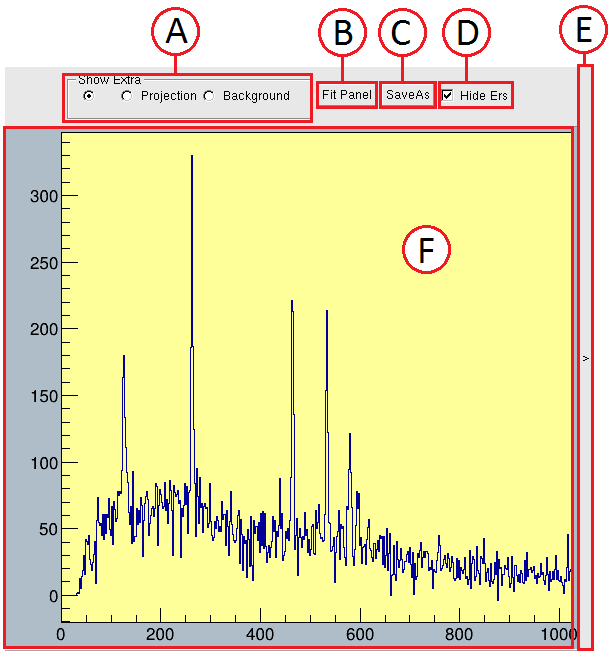
\includegraphics[width=0.5\textwidth]{jGateE.png}
\end{center}
\begin{enumerate}
\item Draw Overlays - Show the total ungated-projection (scaled), or the currently subtracted background spectrum, overlain in the result window.
\item Open Peak Fit Panel - Open an instance of $UltraFitEnv$, the fitting tool is "connected" to the result canvas and will connect with new input if the gate is changed. See Section \ref{sec:peakfit}.
\item SaveAs -Save the histogram currently drawn in the result frame to a file. Opens a dialogue box.
\item Hide Errs - Hide the error bars from background subtraction and draw histogram normally. Note: When selected fits performed with the ROOT FitPanel will not initially display, select the SAME drawing option to fix.
\item Show/Hide Gate Summing Tool.
\item Result Frame. Double clicking in this window will perform a quick Gaussian fit at the cursor and display the centroid.
\end{enumerate}

\subsection{Gate Summing Tool}
The Gate Summing Tool is used for saving the result histograms in memory after gating so that the results of multiple gates can be quickly summed.
\begin{center}
\begin{tabular}{ c c }
\begin{minipage}{0.6\textwidth}
\begin{enumerate}
\item Show/Hide Gate Summing Tool.
\item Create additional save slot.
\item Draw a sum of the selected histograms in the result frame.
\item Delete all histograms in summing tool memory.
\item Sum Check - Use the check marks to selected which saved histograms will be added to the output.
\item Save Buttons - Click to save/overwrite the current gating result histogram to a slot. The button will update with the centroid of the saved gate.
\end{enumerate} \end{minipage}
&
\raisebox{-.5\height}{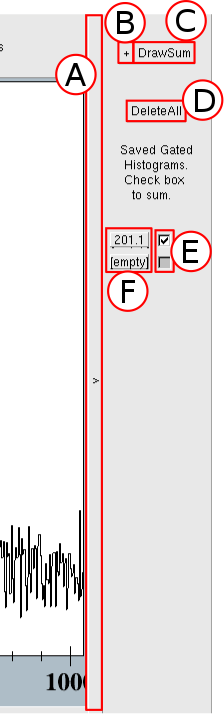
\includegraphics[width=0.2\textwidth]{jGateF.png}}
\\
\end{tabular}
\end{center}


\subsection{3D Gating Window}
For the first gate on a $TH3$ there is significant amount of computation so this is not done live. The output of the first gate is only performed when a new projection is selected, a different background mode is selected or when the [Update] button is pressed.
\begin{center}
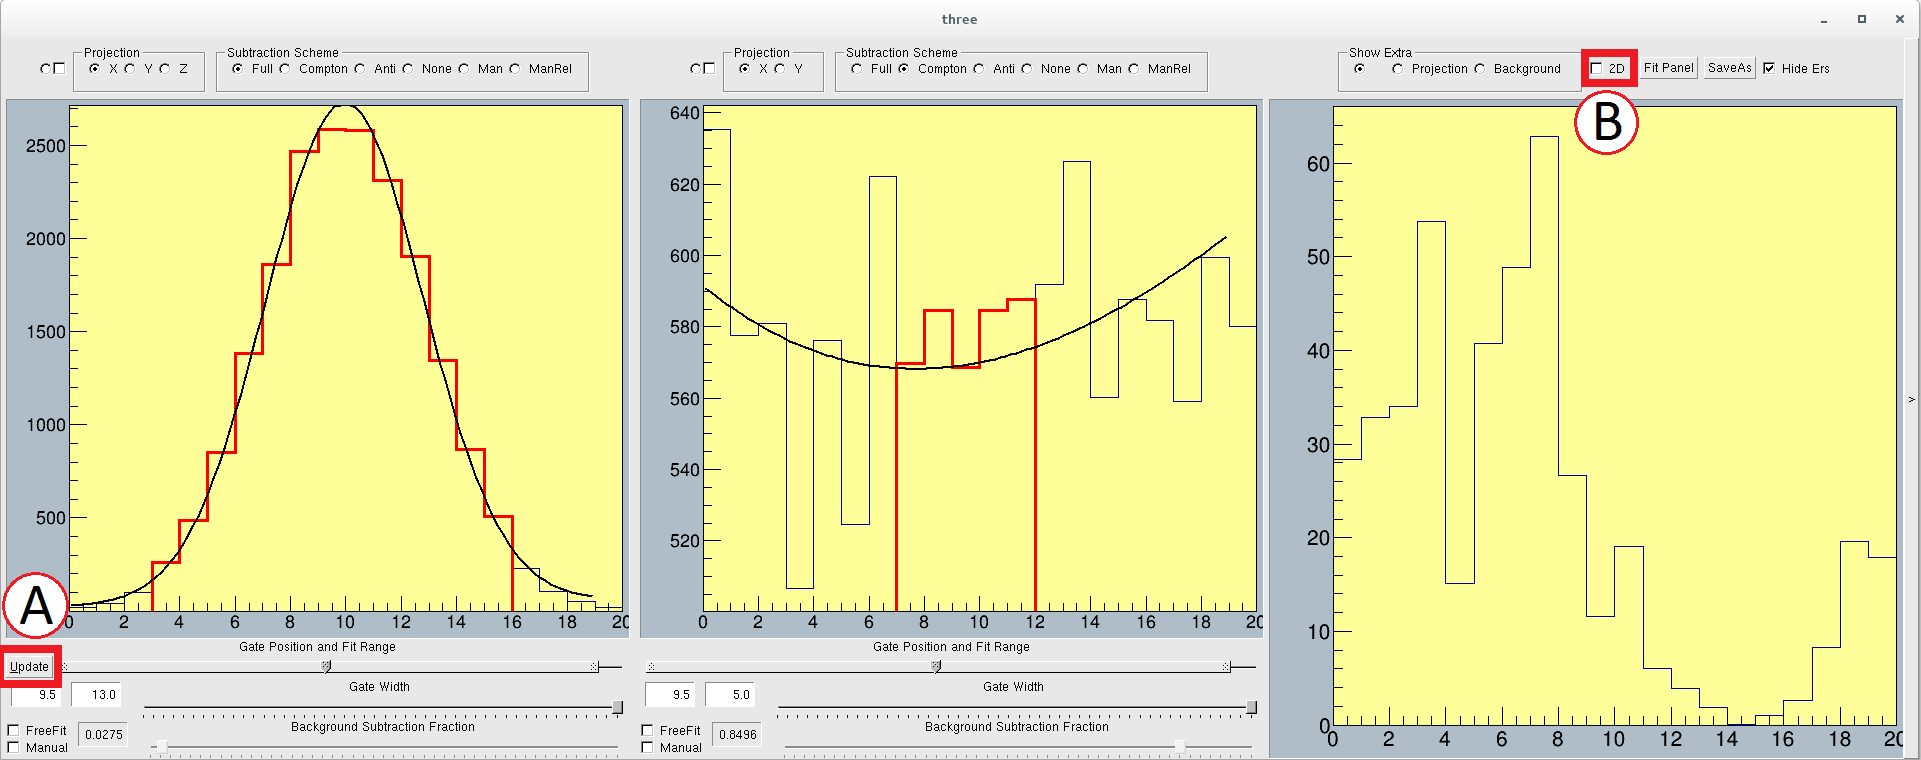
\includegraphics[width=0.95\textwidth]{jGateA.png}
\begin{enumerate}
\item Update - Select after changing gate or background.
\item 2D - Do not perform a second gate but instead pass the TH2 result to the result frame. The gate sum tool can also be used in this mode.
\end{enumerate}
\end{center}


\section{Peak Fitting Tool}\label{sec:peakfit}
The UltraFitEnv fitting environment is designed for the automatic fitting of Gaussian peaks convolved with exponential tails.
The tool has some foibles that are absent from the root fitting environment, but it is far more tuned to the task of fitting spectra and saving the relevant data.
A new instance can be created from the jEnv toolbar or typing:
\lstset{language=C++}
\begin{lstlisting}
new UltraFitEnv();
new UltraFitEnv(TH1*);
new UltraFitEnv(0,TCanvas*);
\end{lstlisting}
The tool operates in two primary modes:
\begin{itemize}
\item A histogram may be captured and stored by the tool.
\item A canvas can be linked to the tool, any new histogram drawn in that canvas will become the fitting target.
\end{itemize}

The fitting tool stores an internal copy of the histogram to avoid empty fitting segfaults. When the tool is "connected" it is to a selected canvas, not to a particular histogram. When a new histogram is drawn in the canvas the fitting tool updates it's internal histogram accordingly. Note: You cannot modify a histogram through the canvas the fitting tool is connected to (as the fitting tool performs $DrawCopy$ of it's internal histogram).

In order to begin fitting click either [$[$Capture Hist$]$ or $[$Link Canvas$]$ and then immediately click on the Canvas/Histogram you want to fit

\subsection{Peak Fitting Controls}
While the mouse pointer is over the fit histogram, the following controls and short-cuts may be used:
\begin{center}
\begin{tabular}{ r l }
$[Left Click]$ & Select peak.\\
$[Ctrl]$ & Set manual bin select (default auto).\\
$[Enter]$ & Fit.\\
$[Middle Click]$ & Select fit-range.\\
$[Shft]$ THEN $[Left$ $Click]$ & Select fit-range.\\
$[Alt]$ THEN $[Left$ $Click]$x2 & Select exclusion region.\\
$[+]$ & Increase the number of peaks.\\
$[-]$ & Decrease the number of peaks.\\
$[0]$-$[9]$ keys & Set the number of peaks.\\
$[.]/[s]/[Del]$ & Save latest fit to list \& histogram.\\
\end{tabular}
\end{center}
  	
\subsection{Peak Fit Function \& Logic}
The tool is designed for fits over small energy regions, as such, all shape parameters of degenerate peaks are shared, as these parameters are dominated by energy dependant physical effects which do not change rapidly. Background across the fit region is approximated by a polynomial + an optional step function constrained by the peak parameters. The step should be used when peak sizes are large compared to background. Pol0, pol1 and pol2 backgrounds may be selected (pol2 are poorly constrained). Watch your fit's Reduced ChiSquards.
\\
\\
For very small numbers of counts the fit mode will automatically switch to Poisson Likelihood fitting rather than Pearson Chi Squared minimisation. Exclusion regions will not function for Likelihood fitting.
\subsection{Fit Inputs}
For multi-peak/degenerate fits peak separation are set rather than absolute centroids. This provides more accurate fitting overall as it is less sensitive to small deviations in the absolute scale i.e. poor calibration. The area ratio between peaks may also be set if it is in known. When inputting multiple peaks to a fit, any constrained peaks should immediately follow the peak to which they are fixed. Un-constrained peaks should be in ascending order.
\lstset{language={}}
\begin{lstlisting}
e.g. We have 3 peaks:
           An unknown ~130 keV, a known 125 keV and a known 145 keV.
           Inputs : A = 125
                    B = A + 20
		    C = 130
          -We set the tool for 3 peaks
          -Enter [20] in to the peak 0-1 "separation" input box.
          -Click on each peak A and C in the histogram window.
          -Click [Fit Peaks].
\end{lstlisting}

For both separation and area ratio between peaks, the box should be left blank to free the fit. Uncertainties on both constraint parameters may also be added in the input box. If no error is given the parameter will be fixed. Plain text input is fairly robust and accepts ENSDF format errors:\\
Example inputs :\quad25.0\qquad0.051(2)\qquad-16.0 5\qquad6+-5\qquad3E-5+3e-6
\\
\\
For problematic fits the shape parameters (Sigma, Decay and Sharing) may be constrained. The bottom most button on the panel [$\wedge$] will expose these options. As with centroid \& ratio these parameters may be fixed or given with uncertainties and should be left blank when not constrained.

\section{Histogram Formatting Functions}

\end{document}
